\section{Interest Flooding in NDN}
\label{sec:interest flooding}

% Points here:
% - Classification
% - Mechanisms: congestion and memory exhaustion
% - Target
% - Effectiveness: random names, non-existing content
% - Assumptions: the network, attackers, attack traffic, and legitimate consumers

%??? - References about other attacks and explicitly stating that this work aims to build a baseline for general Interest Flooding mitigation problem, with other attack profiles and malicious gateways.

\paragraph{Classification}

Interest flooding attack belongs to a class of network-level flooding attacks, where an attacker or a set of distributed attackers inject excessive amounts of Interests in order to overload the network and cause service disruptions for legitimate users (Fig.~\ref{fig:flooding example}).
%
% Definition of service
%
Service for legitimate users is disrupted when the network fails to satisfy Interests either because the Interests did not get through to the data producer or nearby cache, or the Data were lost on the way back to the requester (e.g., because of congested links).

\begin{figure}[htbp]
  \centering
  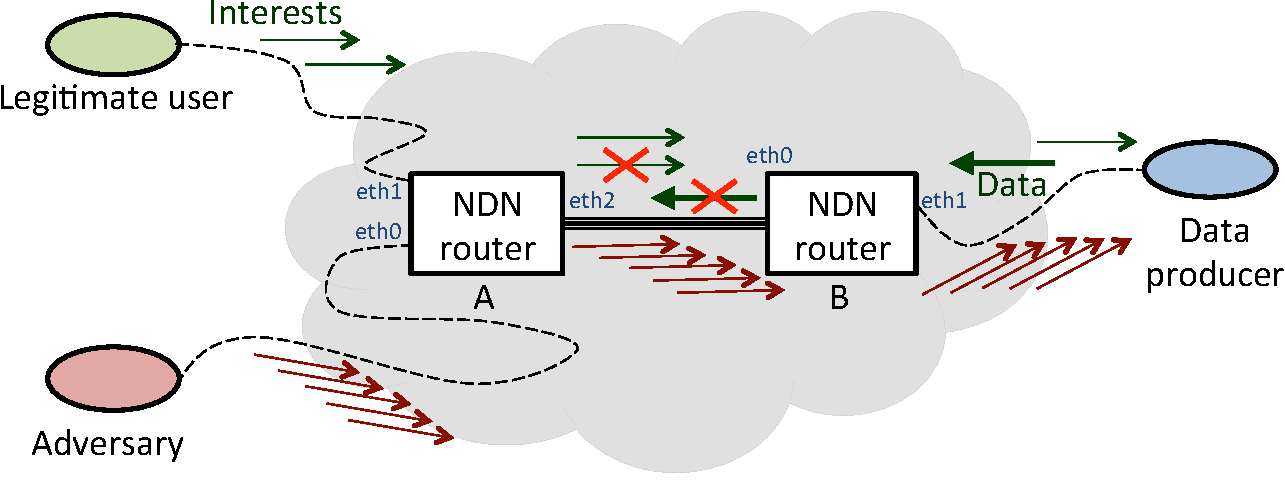
\includegraphics[width=\columnwidth]{attack-definition}
  \caption{Example of the Interest flooding attack}
  \label{fig:flooding example}
\end{figure}

\paragraph{Mechanism}

The Interest flooding attack has two-fold effect on service quality in NDN network: it \textbf{creates network congestion} and \textbf{exhaust resources on routers}.

Like any other packets in the network, malicious Interests consume a portion network capacity.
Thus, a large amount of malicious Interests can lead to network congestion and drop of the legitimate Interests and Data packets.
%  (in case of bidirectional communication)
% The resource exhaustion effect can be much more ???.
% and more critical is the effect on memory and CPU resources of NDN routers.

As NDN routers maintain per-packet states for each forwarded Interest (entry in Pending Interests Table), an excessive volume of malicious Interests leads to creating an excessive number of PIT entries and exhaustion of routers' resources.
When a router has no memory to create a PIT entry for an incoming Interest, it drops this Interest.
% there is no point in forwarding the Interest further.
% Otherwise, if Data comes back, it would be considered unsolicited and dropped anyways.
Therefore, the routers' memory exhaustion effect may disrupt service for legitimate users even without causing network congestion, if the router has limited memory resources.

\paragraph{Target}

Because communication in NDN is content-centric, it is impossible for an adversary to target specific routers or end-hosts, as neither of them have a global network identity.
However, an adversary can target a specific namespace, which in NDN network can loosely correspond to a network location or sets of network locations.
For example on Fig.~\ref{fig:flooding example}, if the Data producer is the exclusive owner of \ndnName{/foo/bar} namespace and is single-homed to router B, both router B and the Data producer would receive all Interests for \ndnName{/foo/bar/\ldots} that cannot be otherwise satisfied from in-network caches.
It should be noted that if connectivity in NDN network is rich (users are multi-homing to many providers, many interconnections between providers), targeting of specific locations is largely unfeasible, as stateful Interest forwarding strategy in NDN can fully and effectively utilize multiple available paths to destination~\cite{adaptive-forwarding}.

% \paragraph{Countermeasures}?

\paragraph{Effectiveness}
% Эффективность атаки

To efficiently implement the Interest flooding attack, an adversary needs to make sure that (1) the expressed Interests are getting as close to the Data producer as possible, as well as (2) the corresponding PIT entry (state) is kept on NDN routers for as long as possible.
In order to achieve effectively the first requirement, the malicious Interests should avoid collapsing and cache hits.
To keep PIT entry for a prolonged period of time, the malicious Interests should not bring any data.%
\footnote{While NDN allows users to specify lifetime of the Interest inside the Interest packet~\cite{ndn-conext,ndn-tr}, it is router's decision for how long it is willing to keep the PIT entry.  For example, and we assume this in the rest of the paper, the maximum time for which any Interest is admitted is one second.} 

In other words, to maximize effect of the attack, each malicious Interest generated by individual attack bots should have a unique name and should not correspond to any existing data (\emph{unique junk Interests}).

\paragraph{Assumptions}
% - assumptions about attacker position
% - assumptions about the producer / producer namespace
% - assumptions about the attack traffic / attack pattern

In this paper we are making the following assumptions about the Interest flooding attack:
\begin{itemize}
\item only client nodes can be compromised and become attack bots;
\item there are no colluding attackers inside the Data producer's network; and
\item the attack is carried only using unique junk Interests.
\end{itemize}

We also assume that NDN forwarding strategy uses only single-path Interest forwarding, always choosing the best-metric route advertised by the routing protocol.
This way, we are able to analyze the attack in its best environment, as enabling the multi-path forwarding would only alleviate effects of the Interest flooding attack.


% Though NDN is capable of multipath Interest forwarding and forwarding strategy switching, we are using Best Route (single path) forwarding strategy in all of our experiments. 

\paragraph{Disclaimer}

In this paper we are not trying to completely solve all denial of service problems that can be caused by various variations of the Interest flooding attack.
Our primary focus is to demonstrate that while NDN opens doors to new types of denial of service attacks, stateful packet forwarding of NDN makes it possible to mitigate such attacks, adding little additional complexity to the network.
In section~\ref{sec:discussion} we discuss our choice of the assumptions in more detail, as well as discuss potential of the Interest flooding attack under several other attack assumptions.


%%% Local Variables: 
%%% mode: latex
%%% TeX-master: "paper"
%%% End: 
